% lintrans - The linear transformation visualizer
% Copyright (C) 2021-2022 D. Dyson (DoctorDalek1963)

% This program is licensed under GNU GPLv3, available here:
% <https://www.gnu.org/licenses/gpl-3.0.html>

\documentclass[../development.tex]{subfiles}

\begin{document}

Now that I've got \texttt{v0.2.2} working and released, it's time to talk to some teachers. Ms Arnold is going to be the one that's actually using it, so obviously I needed to talk to her about it, but she wasn't available for a few days. I was talking to another maths teacher, Mr Dunkley, about my personal statement and took the opportunity to show him \texttt{lintrans} as well.

He was able to download and run it on a native Windows 10 installation, which was quite a relief. I'd been unable to test it on a real bare-metal Windows installation so far; I only had virtual machines.

He suggested two main improvements: \begin{enumerate}
	\item In the visual definition dialog, the basis vectors should snap to integer coordinates when they get close enough
	\item There should be a dialog box which displays matrices that you've already defined
\end{enumerate}

\subsubsection{Fixing a bug with animating stretches\label{development:teacher-suggestions:fixing-a-bug-with-animating-stretches}}

While Mr Dunkley was playing around with \texttt{lintrans}, I noticed a bug where animating uniform stretches, where every direction gets stretched equally work, just fine, but a matrix like $\begin{pmatrix}3 & 0\\ 0 & 1\end{pmatrix}$ would be animated as if it was $\begin{pmatrix}3 & 0\\ 0 & 3\end{pmatrix}$ and the plane would stretch equally in all directions.

After looking at the code later, I realised this was a problem with my new animation code detecting this type of matrix as a rotation. To fix this, I could just add a check to the \texttt{if} statement before the rotation animation code. This new check would make sure that the basis vectors of the application matrix were approximately the same length. By checking this as well, I fixed the bug.

%: eb118f02db9fb9c76ce15a976f81a037415d2a4e
%: src/lintrans/gui/main_window.py:410-417 highlight=417

\subsubsection{Fixing a hang after closing during an animation\label{development:teacher-suggestions:fixing-a-hang-after-closing-during-an-animation}}

This bug was tiny and only really affected me, but when I run \texttt{lintrans} from the terminal with \mintinline{sh}{python -m lintrans} and close it during an animation, I have to wait a moment to get my shell prompt back. Clearly, the program is still running even after the main window is closed.

I'm not entirely sure what was happening here, but it was something to do with Qt5's event loop and threading model, and I could fix the bug by just overriding \pyinline{LintransMainWindow.closeEvent()} to set \pyinline{self.animating = False} and that would ensure that animations are stopped before the main window closes.

%: d60c1878058799be544f5cf0847b478dccd3a021
%: src/lintrans/gui/main_window.py:262-265

\subsubsection{Adding snapping in the visual definition dialog\label{development:teacher-suggestions:adding-snapping-in-the-visual-definition-dialog}}

I was now ready to implement snapping in the visual definition dialog.

The \pyinline{DefineVisuallyWidget} class has a \pyinline{self.dragged_point} attribute, which is the coordinates of the point being dragged. In \pyinline{mouseMoveEvent()}, we get the coordinates of the current cursor position and set the dragged point accordingly. That's all that happens in the old code.

%: d60c1878058799be544f5cf0847b478dccd3a021
%: src/lintrans/gui/plots/widgets.py:127-147

To add snapping to this, we can just get the 4 integer coordinates around the dragged point, check each of their distances to the dragged point, and if it's sufficiently close to one of them, snap it to that point.

%: f2de39fec299bb8ed155ee649d34c9063787e71a
%: src/lintrans/gui/plots/widgets.py:128-165

This all worked very well.

\subsubsection{Respecting transitional animation in animation sequences\label{development:teacher-suggestions:respecting-transitional-animation-in-animation-sequences}}

It's good to animate a sequence of matrices by applying them one after another, but it can also be beneficial to animate a sequence by just moving between them in a transitional animation style. This is already possible for individual animations by disabling the \textit{Applicative animation} display setting, but it would be nice to respect this setting for animation sequences.

To do this, I just have to add a few lines to the part where we do animation sequences.

%: 41907b81661f3878e435b794d9d719491ef14237
%: src/lintrans/gui/main_window.py:339-367 highlight=348-351

\subsubsection{Adding the info panel\label{development:teacher-suggestions:adding-the-info-panel}}

One of things that Mr Dunkley wanted to see was a panel or dialog box that would display all the matrices that you've already defined.

\paragraph{Creating the initial dialog\label{development:teacher-suggestions:adding-the-info-panel:creating-the-initial-dialog}}

The first thing I did was create a new git branch, and then I created a new dialog class, added a button to display the new info panel, and created a simple utility method for a \pyinline{MatrixWrapper} to return a list of all the matrices it's got defined.

%: 6469f9f3678a89b3b7f388a6c5132335d9a6a947
%: src/lintrans/matrices/wrapper.py:251-263

%: 6469f9f3678a89b3b7f388a6c5132335d9a6a947
%: src/lintrans/gui/dialogs/misc.py:100-110

%: 6469f9f3678a89b3b7f388a6c5132335d9a6a947
%: src/lintrans/gui/main_window.py:203-208

Trying to open the new info panel results in a tiny, useless dialog box appearing but the defined matrices get printed out in the terminal, which is exactly what I expected. It's a good proof of concept, but obviously needs a bit of visual polish.

\begin{figure}[H]
	\centering
	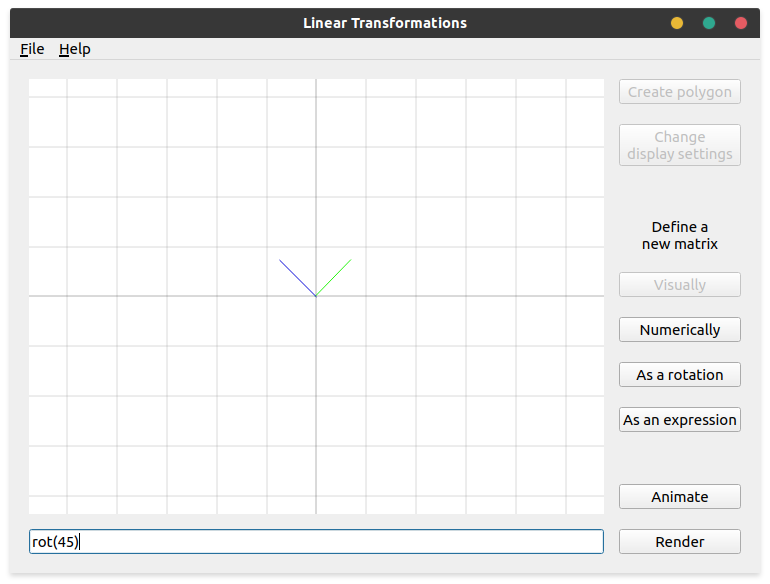
\includegraphics[width=0.95\linewidth]{development/6469f9f3678a89b3b7f388a6c5132335d9a6a947/gui.png}
	\caption{The GUI with the tiny dialog box and new button visible in the background}
	\label{fig:development:6469f9f3678a89b3b7f388a6c5132335d9a6a947:gui.png}
\end{figure}

\paragraph{Adding the matrices to the panel\label{development:teacher-suggestions:adding-the-info-panel:adding-the-matrices-to-the-panel}}

The next step was obviously to add the widgets that actually represent these matrices in the dialog box. To do this, I created a layout and iterated over the matrices in the wrapper to add some widgets for each. These widgets consist of a name label, a label for \enquote{=}, and a container widget to display the content of the matrix. I created a separate method to generate a container widget for the matrix content.

%: addc22a8984a9d8e1d100b5800836a2af3f42760
%: src/lintrans/gui/dialogs/misc.py:102-183

\fsbsr[0.3]{development/addc22a8984a9d8e1d100b5800836a2af3f42760/info-panel.png}{The info panel with some defined matrices, and the parentheses not working correctly}{This container widget uses a grid layout to have the numbers arranged correctly, as well as stretching the parentheses either side to properly cover the numbers.\par However, the parentheses don't stretch properly. I also get the message \enquote{QGridLayout: Multi-cell fromCol greater than toCol} in the terminal whenever I open the info panel. One for each matrix defined numerically. Suffice to say, this is not what I was trying to do.}

\paragraph{Fixing alignments and stretches\label{development:teacher-suggestions:adding-the-info-panel:fixing-alignments-and-stretches}}

After checking the documentation for the \texttt{QGridLayout::addWidget()} function\cite{qt5-docs-qgridlayout-addwidget} and experimenting with some different numbers, I fixed the row and column numbers for the parentheses. I also created a temporary font for the parentheses to make them bigger. I had to make them thinner as well to avoid them looking weird. I also made the matrix names bold.

%: 63279a27ac6fa86061c4ba10152244b2bb4ced87
%: src/lintrans/gui/dialogs/misc.py:102-191

\begin{figure}[H]
	\centering
	\includegraphics[width=0.4\linewidth]{development/63279a27ac6fa86061c4ba10152244b2bb4ced87/info-panel.png}
	\caption{The new and improved info panel with correct alignment and stretching}
	\label{fig:development:63279a27ac6fa86061c4ba10152244b2bb4ced87:info-panel.png}
\end{figure}

\paragraph{Arranging matrices in multiple columns\label{development:teacher-suggestions:adding-the-info-panel:arranging-matrices-in-multiple-columns}}

The only remaining problem with the info panel is that it just extends into one long vertical column as more matrices are added. Obviously there are 26 letters in the alphabet, so 26 possible matrices that can be defined. However, 26 is a semiprime, which means if I want to arrange the matrices in a rectangle, I have to do $2 \times 13$ or $13 \times 2$. This is not particularly useful. Instead, I think it would be better to have an arrangement closer to a square, which a few matrices extra at the end. I'll go with 4 rows of columns with 6 matrices each and an extra column at the end for the last 2 matrices if necessary.

To do this, I just use the index of the current matrix to set the column for that matrix. Qt5's grid layout handles spacing and creating extra columns for me, so I just have to work out which column to put each matrix in.

%: 8e0f2dfe27fb9629b0f8cd33a25a61f85b5443e8
%: src/lintrans/gui/dialogs/misc.py:120-151

\begin{figure}[H]
	\centering
	\includegraphics[width=0.98\linewidth]{development/8e0f2dfe27fb9629b0f8cd33a25a61f85b5443e8/info-panel.png}
	\caption{The info panel with all matrices defined, arranged in multiple columns}
	\label{fig:development:8e0f2dfe27fb9629b0f8cd33a25a61f85b5443e8:info-panel.png}
\end{figure}

\subsubsection{Fixing a bug with matrices with a 0 column\label{development:teacher-suggestions:fixing-a-bug-with-matrices-with-a-0-column}}

Currently, if you set one basis vector to $\mathbf{0}$, then it will continue to draw the line for the zeroed basis vector. This doesn't make much sense, since the non-zero basis vector is the only one that has an impact on the matrix. To fix this, I can just check for a zero column and not draw the vector lines in that case.

%: 37abc3dbb5d99c9ec812e6c887fc6c021f9c91c6
%: src/lintrans/gui/plots/classes.py:244-272

\begin{figure}[H]
	\begin{minipage}{0.48\linewidth}
		\centering
		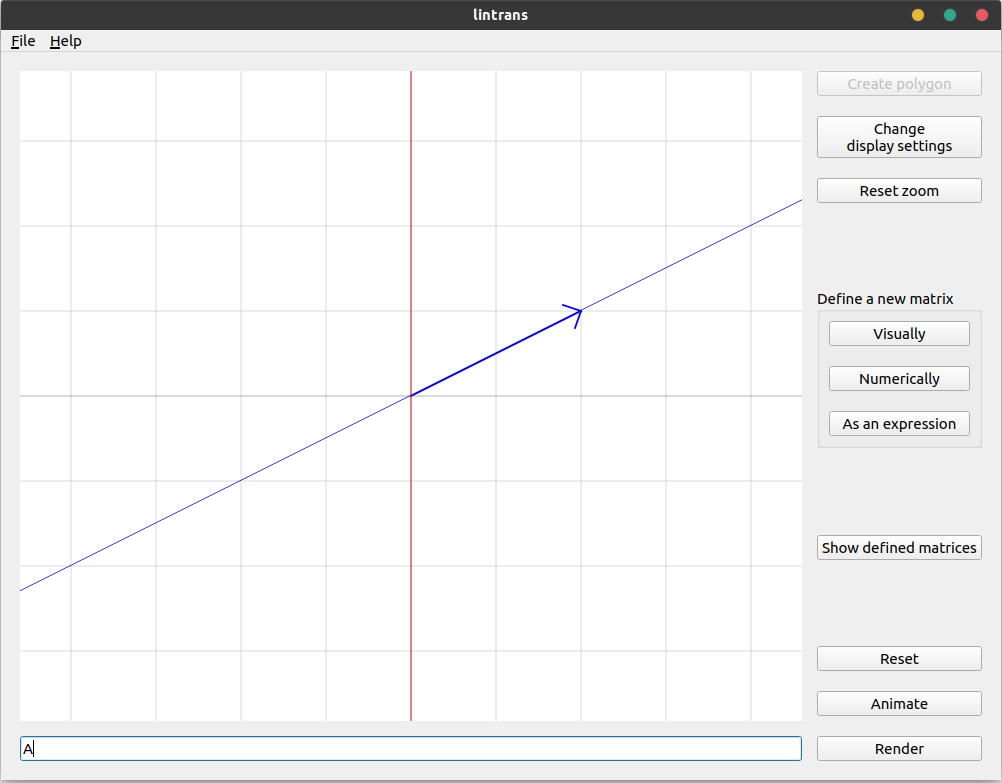
\includegraphics[width=\linewidth]{development/37abc3dbb5d99c9ec812e6c887fc6c021f9c91c6/before.png}
		\caption{Before the bug fix}
		\label{fig:development:37abc3dbb5d99c9ec812e6c887fc6c021f9c91c6:before.png}
	\end{minipage}\hfill
	\begin{minipage}{0.48\linewidth}
		\centering
		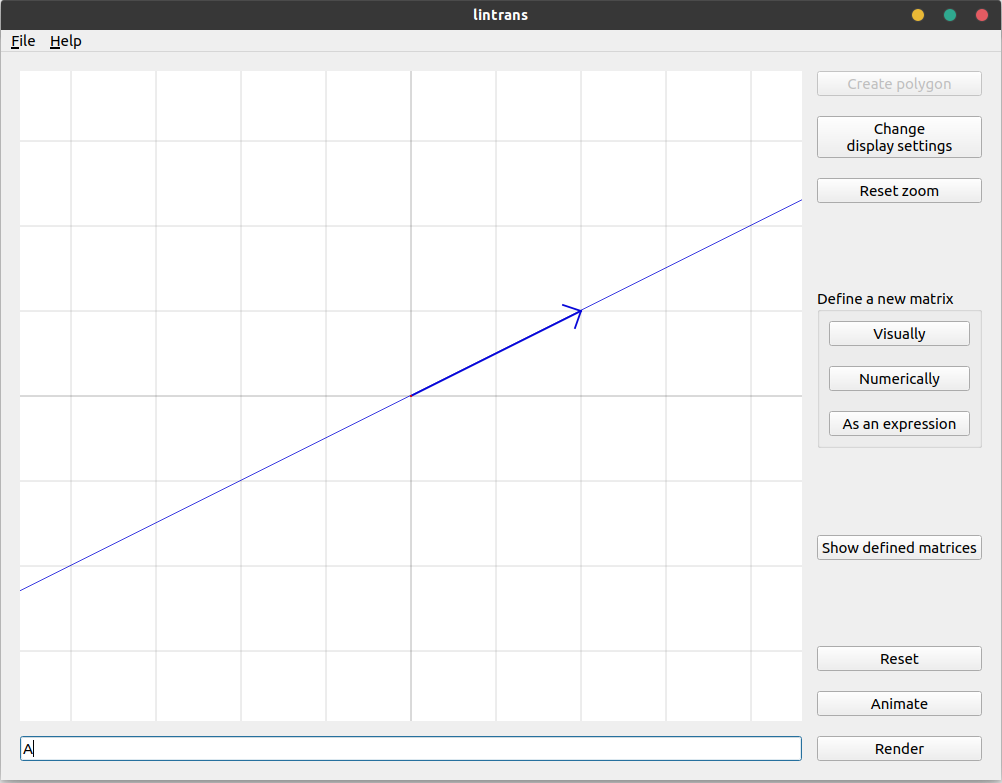
\includegraphics[width=\linewidth]{development/37abc3dbb5d99c9ec812e6c887fc6c021f9c91c6/after.png}
		\caption{After the bug fix}
		\label{fig:development:37abc3dbb5d99c9ec812e6c887fc6c021f9c91c6:after.png}
	\end{minipage}
\end{figure}

\end{document}
